% =====================================================================
%  Appendix C -- Simulation details (owner: SIM).
%  Source of truth: results/sim_results.json (meta.configs, meta.runtime_s).
%  The history of superseded runs is in code/README.md (Run history), not here.
% =====================================================================
\providecommand{\simfit}[1]{\resizebox{\ifdim\width>\linewidth\linewidth\else\width\fi}{!}{#1}}
\providecommand{\Sp}{\mathrm{Sp}}
\providecommand{\Se}{\mathrm{Se}}
\section{Simulation details}\label{app:simdetails}

This appendix documents the simulation study of \cref{sec:simulation}. All data are synthetic. The catalogue, the classifier, the personas and the users are generated from random numbers and invented parameters, and no real platform, item or user is represented. The source of truth is \texttt{results/sim\_results.json}, which records the configurations (\texttt{meta.configs}), the seeds, the software versions and the runtimes of every run, as well as the results. \texttt{results/SUMMARY.md} prints the same values, formatted by \texttt{code/write\_summary.py}. The code is the package \texttt{code/ampsim} (version 1.0.0), with modules for the catalogue and classifier (\texttt{world}), the recommender and the accounts (\texttt{engine}), validation and correction (\texttt{measurement}), the double-sampled exposure of the protocol (\texttt{doublesample}), Markov chains (\texttt{markov}) and confidence sequences (\texttt{sequential}), and the scripts \texttt{run\_experiments.py}, \texttt{make\_figures.py} and \texttt{write\_summary.py}.

\subsection{Configuration}\label{app:sim-config}

\Cref{tab:sim-config} lists the parameters of the synthetic world, and \cref{tab:sim-personas} the four synthetic personas. The codes P1--P4 are used in every figure, table and paragraph of \cref{sec:simulation}, so that no panel can be read as a finding about a real group of users. Three mechanisms need more detail than the tables give.

\paragraph{Catalogue} An item of topic $t$ and type $j$ has the embedding $x_c=(e_t+a_j e_A+0.35\,\epsilon_c)/\|e_t+a_je_A+0.35\,\epsilon_c\|$, where $e_t$ is the direction of topic $t$, $e_A$ the antisemitism direction, $a_j$ the loading of the type and $\epsilon_c$ standard normal in eight dimensions. The numbers of borderline and antisemitic items in each topic are proportional to the topic's size and to its relative propensity, scaled so that $4\%$ of all items are antisemitic and twice as many are borderline. Half of the antisemitic items are coded. Each item also has an engagement prior (``bait''), a background popularity $w_c$ (log-normal, with a loading on bait) and a posting rate (log-normal, with a multiplier by type). The persona seed pool is the set of the $200$ neutral items most similar to the persona's taste vector. No seed is borderline or antisemitic.

\paragraph{Popularity and load} Global popularity is $p_c=Vw_c$ when it is frozen, where $V$ is the background volume of openings per round. In E2 it is updated after every round as $p\leftarrow\delta p+(1-\delta)(Vw+o)$, where $o$ counts the puppets' openings in the round and $\delta=0.5^{1/100}$, a half-life of one day of $100$ rounds. Between sessions the remaining rounds of the day pass with $o=0$. For a target traffic share $\rho$, $V=n(1-\rho)/\rho$, where $n$ is the number of puppets and sentinels. The realised traffic share is the puppets' openings divided by those openings plus $V$ times the number of active rounds. The load is the puppets' share of the engagement with the items they opened, $\sum_co_c/\sum_{c:o_c>0}(o_c+Vw_c\,r)$ over the $r$ active rounds of a wave, averaged over waves.

\paragraph{Evolving demand} After each formation session in E3, a user's taste moves toward the mean embedding of the items opened, $\theta\leftarrow(1-0.05)\theta+0.05\,\bar x$, renormalised. For $x\in\{\mathsf B,\mathsf A\}$, the appetite becomes $\alpha_x+0.4f_x-0.1\{\alpha_x-\alpha_x(0)\}$, capped at $2$, where $f_x$ is the share of the session's openings in state $x$. The share of the eligible pool drawn from followed borderline and antisemitic items becomes $s+0.02(f_{\mathsf B}+f_{\mathsf A})-0.1\{s-s(0)\}$, clipped to $[0,0.5]$; it starts at zero. Real users start from their persona's taste and appetites plus normal noise (s.d.\ $0.15$ on taste, then renormalised, and $0.3$ on the appetites for $\mathsf B$ and $\mathsf A$), with new accounts ($v_u=0$) and no training.

\begin{table}[tp]
\centering
\caption{Configuration of the synthetic world (\texttt{meta.configs} of \texttt{results/sim\_results.json}). All values are invented. Topic order: news, sport, entertainment, culture and community, regional news, conspiracy; these are labels of invented clusters of items. Type order: neutral, borderline, coded antisemitic, explicit antisemitic. The personas are in \cref{tab:sim-personas}.}\label{tab:sim-config}
\footnotesize
\setlength{\tabcolsep}{4pt}
\renewcommand{\arraystretch}{1.0}
\begin{tabularx}{\textwidth}{@{}>{\raggedright\arraybackslash}p{6.2cm}>{\raggedright\arraybackslash}X@{}}
\toprule
Parameter & Value \\
\midrule
\multicolumn{2}{@{}l}{\emph{Catalogue}} \\
Items; embedding dimension & $5{,}000$; $8$ \\
Topic shares of items & $0.30$, $0.18$, $0.18$, $0.08$, $0.11$, $0.15$ \\
Propensity of borderline and antisemitic items by topic & $0.4$, $0.1$, $0.1$, $1.0$, $1.5$, $2.0$ \\
Antisemitic share; borderline-to-antisemitic ratio; coded share & $0.04$; $2$; $0.5$ \\
Loading $a_j$ on $e_A$ by type; embedding noise s.d. & $0$, $0.5$, $0.7$, $1.4$; $0.35$ \\
Bait: mean by type; s.d. & $0$, $0.5$, $0.4$, $0.3$; $0.3$ \\
Background popularity: s.d.\ of log; loading on bait & $1.0$; $1.0$ \\
Posting rate: multiplier by type; s.d.\ of log & $1$, $1.2$, $1.3$, $1.5$; $0.5$ \\
Item neighbours; persona seed pool & $15$; $200$ neutral items \\
\addlinespace[2pt]
\multicolumn{2}{@{}l}{\emph{Recommender}} \\
Eligible pool; trending candidates; slate $k$ & $50$; $15$; $4$ \\
Algorithmic score: weights on $\langle v_u,x_c\rangle$, log popularity, bait; Gumbel scale & $2.0$, $0.3$, $1.0$; $0.5$ \\
Embedding update $v_u\leftarrow(1-\lambda)v_u+\lambda x_c$ & $\lambda=0.1$ \\
Popularity-only feed: Gumbel scale & $0.05$ \\
\addlinespace[2pt]
\multicolumn{2}{@{}l}{\emph{Choice and sessions}} \\
Protocol puppets: $s_{\mathrm{safe}}$; similarity threshold & $-0.5$; $0.25$ \\
Naturalistic: weights on taste, bait, position, current item & $3.0$, $0.8$, $-0.3$, $2.0$ \\
Naturalistic: utility of opening nothing & $1.0$ (E3); $-50$, so never (E4) \\
Training: days $\times$ seeds per day; seeds drawn per puppet & $3\times10$; $30$ \\
Measurement: sessions $\times$ steps $T$; rounds per day & $10\times20$ ($4$ of the $10$ in E4b, E5b); $100$ \\
\addlinespace[2pt]
\multicolumn{2}{@{}l}{\emph{Demand evolution (E3)}} \\
Taste drift; appetite gain, decay, cap & $0.05$; $0.4$, $0.1$, $2.0$ \\
Followed-fringe gain, decay, cap & $0.02$, $0.1$, $0.5$ \\
\addlinespace[2pt]
\multicolumn{2}{@{}l}{\emph{Classifier regimes: flag rate by type}} \\
ND, non-differential & $0.02$, $0.02$, $0.85$, $0.85$ \\
DU, borderline false positives & $0.01$, $0.40$, $0.85$, $0.85$ \\
DD, coded false negatives & $0.02$, $0.02$, $0.35$, $0.95$ \\
NDI, item-level noise & as ND in expectation; realised $0.016$, $0.023$, $0.86$, $0.79$ \\
\bottomrule
\end{tabularx}
\end{table}

\begin{table}[tp]
\centering
\caption{The synthetic personas and their codes. Each is a demand profile in the invented catalogue: weights over its topics (\cref{tab:sim-config}), which set the eligible pool and the seed items, and appetites, utility shifts for the content states $(\mathsf N,\mathsf B,\mathsf A)$ used only by naturalistic accounts (E3, E4). The second column names the candidate persona of \cref{sec:prot-personas} for which each profile stands in; no profile describes a real group of users. Antisemitic share: share of antisemitic items among the topics followed, weighted by the topic weights. $\mu_{\mathrm{ref}}$: impression exposure of protocol puppets under the reverse-chronological feed, regime ND (E1 pools).}\label{tab:sim-personas}
\footnotesize
\setlength{\tabcolsep}{4pt}
\begin{tabularx}{\textwidth}{@{}l>{\raggedright\arraybackslash}p{2.6cm}>{\raggedright\arraybackslash}Xcccc@{}}
\toprule
Code & Stands in for & Synthetic demand profile: topic weights & Appetites & Antisemitic share & $\mu_{\mathrm{ref}}$ & E3 share \\
\midrule
P1 ($d_0$) & General interest (baseline) & three broad topics: news $1$, sport $0.8$, entertainment $0.8$ & $(0,-0.5,-2.5)$ & $0.012$ & $0.018$ & $0.6$ \\
P2 & Jewish interest & culture and community $1$, news $0.4$, entertainment $0.25$ & $(0,-1.0,-4.0)$ & $0.041$ & $0.054$ & $0.1$ \\
P3 & Middle East news & regional news $1$, news $0.5$, culture and community $0.2$ & $(0,0,-2.0)$ & $0.064$ & $0.082$ & $0.15$ \\
P4 & Conspiracy-adjacent & conspiracy $1$, news $0.3$, regional news $0.25$ & $(0,0.5,-1.0)$ & $0.092$ & $0.113$ & $0.15$ \\
\bottomrule
\end{tabularx}
\end{table}

\subsection{Experiments}\label{app:sim-experiments}

\paragraph{E1} For each of the four regimes, one pool of $1{,}000$ protocol puppets per persona and policy (algorithmic, reverse-chronological, random, popularity-only), simulated in chunks of $1{,}000$ accounts with popularity frozen. The pools are saved in \texttt{results/raw/pool\_<regime>.npz} as per-puppet impression counts by true type and score band. An audit draws $U\in\{5,10,20,40,80\}$ puppets per cell with replacement, $R=1{,}000$ times. Its validation sample draws $100$ impressions per score band and arm without replacement (all of a band if it has fewer), for $500$ per arm; $250$ and $1{,}000$ are also run with $U=20$. Pooled error rates are estimated from both arms' samples, weighted by inverse inclusion probabilities. The variance of the corrected estimators is computed by the delta method from the between-puppet covariance of the band shares and binomial variances, with the finite-population correction, for the validated band prevalences. The true $\mathrm{AR}$ and $\mathrm{AA}$ are those of the pools, with Monte Carlo standard errors.

\paragraph{E1b} For each variant, $1{,}000$ protocol puppets per persona and arm (algorithmic and reverse-chronological), recording the true and flagged shares of each of their $10$ sessions; in the bucket variant every account has a shift drawn from $\mathrm N(0,1)$ that is added to the algorithm's weight on bait. Audits draw $U\in\{10,20,40\}$ puppets per cell, $R=2{,}000$ times. Known error rates are the realised exposure-weighted rates of the pool, pooled over the arms or by arm. External validation draws $\widehat\Se$ from $\mathrm{Bin}(300,\Se)/300$ and $\widehat\Sp$ from $\mathrm{Bin}(1{,}500,\Sp)/1{,}500$, pooled or separately per arm, and uses the variances \eqref{eq:mc-varAA}--\eqref{eq:mc-varAR} or those of \cref{thm:misclass}(d).

\paragraph{E2} Three designs, each with $15$ protocol puppets per persona and arm (algorithmic, reverse-chronological and popularity-only) and $8$ untrained sentinels with P1's follow profile on the algorithmic feed: simultaneous (seed pool of $40$ items, one wave); low co-viewing (seed pool of $200$, one wave); staggered (seed pool of $40$, five waves with gaps of five days). The simultaneous design is run at traffic shares $0$, $0.02$, $0.05$, $0.1$, $0.2$ and $0.3$, the other two at $0$, $0.1$ and $0.3$, each with $R=24$ replications. Baseline sentinels are measured before each audit without feeding popularity. The randomised-saturation estimates pair replication $i$ at the lower share with replication $i+12$ (modulo $24$) at the higher share, so that the two audits are independent. The slopes $\xi$ are the largest ratios of $|\text{shift}|$ to load over the grid. The sensitivity interval of \cref{prop:interference}(d) uses $\xi_\Delta$ at this simulated value, an oracle that no audit observes (\texttt{E2.sensitivity\_xi\_source} in the JSON).

\paragraph{E3} $3{,}000$ real users and two formed copies, as in \cref{sec:sim-decomp}, with checkpoints at $H\in\{3,10,20,40\}$ sessions. At each checkpoint, each copy is evaluated for three sessions under each policy (four cells), and a fixed-demand counterpart of each cell (the user's current demand held fixed, a new account, three burn-in and three evaluation sessions) checks \cref{asm:demand}. Standard errors are delta-method standard errors over users. The persona-contrast decomposition and the protocol-puppet audit use the ND pool of E1.

\paragraph{E4} Base runs: $250$ untrained naturalistic accounts per persona and policy (algorithmic, reverse-chronological), three burn-in sessions, ten estimation sessions of $20$ steps and one session of $200$ steps. Perturbation runs use the algorithmic policy only. In the tilt runs the algorithm's score of every item with $L_c=1$ is raised by $\varepsilon\in\{0,0.1,0.25,0.5,1\}$. In the replacement runs the opened item is replaced by a uniformly drawn antisemitic item with probability $\varepsilon\in\{0,0.01,0.02,0.05\}$. Transition matrices are maximum-likelihood estimates over the states of consumed items; a row without departures takes the pooled next-state distribution. Bootstrap standard errors resample accounts ($200$ resamples).

\paragraph{Detailed pools} E4b, E5b and E5s use the E1 pools of regimes ND, DU and DD, re-simulated with the same seeds and chunks while recording, for the algorithmic and reverse-chronological puppets, per-session impression counts by type and score band, the type and band of every opened position, and slate states (\texttt{results/raw/pool\_detail\_<regime>.npz}). The recording draws no random numbers; the counts are identical to the E1 pools and the per-session counts add up to them (\texttt{E5b.pools} in the JSON). After its ten sessions, every puppet runs one further session of $200$ steps.

\paragraph{E4b} For each regime, persona and arm, the true slate state of a step is the most severe true state among its $k=4$ positions, and the observed state is $\mathsf A$ if a position is flagged, else $\mathsf B$ if a position lies in score band $[-1,0)$, else $\mathsf N$. Chains are estimated from the transitions and first states of the $10$ sessions of all $1{,}000$ puppets, as three-state chains and collapsed to $\{\mathsf A,\text{not }\mathsf A\}$. Predictions on the impression scale multiply slate functionals by $\bar k_{\mathcal A}/k$, with $\bar k_{\mathcal A}$ ($1.02$--$1.26$) from the same sessions. The correction inverts the slate confusion matrix $C$ in $C^{\top}\operatorname{diag}(\bm\nu)PC$ (\cref{prop:markov-mle}), sets negative entries to zero and renormalises the rows. Item-level confusion is the cell's known exposure-weighted rate of each observed class by true state. Under the protocol's approximation, a slate not in $\mathsf A$ is read as $\mathsf A$ with probability $1-\Sp^k$ and a slate in $\mathsf A$ with probability $1-(1-\Se)\Sp^{k-1}$; with the true composition, the rows average over the simulated joint distribution of the numbers of borderline and antisemitic positions per slate. The three-state correction is computed only where the condition number of $C$ is below $100$. Long-run targets are the shares in steps $100$--$199$ of the $200$-step session. Replications: $120$ puppets per arm drawn with replacement, each with four of its sessions drawn without replacement, $R=500$.

\paragraph{E5b} For each persona, regime (ND, DD) and case (true arms; null, both arms from the reverse-chronological pool), $R=2{,}000$ audits of $120$ pairs, each puppet drawn with replacement from the detailed pool with four of its ten sessions drawn without replacement. Codes per puppet: $\min(10,\cdot)$ flagged positions; $\min(5,\cdot)$ opened positions (never flagged under the avoid-on-flag rule, as the code checks); $20$ other unflagged positions over score bands $0$--$2$, allocated by D'Hondt rounding of $20\,n_hs_h/\sum_jn_js_j$ with at least one per non-empty band, where $s_h=\{f_h(1-f_h)\}^{1/2}$ and $f_h$ is the false-omission rate of band $h$ among non-opened positions, pooled over the regime's personas and arms ($s_h=0.014$, $0.070$, $0.285$ under ND and $0.070$, $0.173$, $0.354$ under DD). Within a stratum the coded positions are a simple random sample, so true positives are hypergeometric. Sequences: \cref{alg:sequential} with $\lambda=1$ and its version for pair differences, with $b\in\{0,1\}$; betting sequences of \cref{thm:sequential}(b) on a grid of $300$ log-spaced ratios in $[0.1,10]$ and of $801$ values of $\mathrm{AA}$ in $[-0.1,0.1]$. Coverage is evaluated at the ends of waves. The closed form is $V^{\mathrm{ds}}+nV^{\mathrm{ds}}_{\mathrm{val}}$ of \cref{sec:prot-sizes} with the pool's $\mu$, $q$, $\Se$, $\Sp$, $\PPV$ and $\FOR$, $kTS=320$, and the simulated variance of a puppet's true exposure. \emph{Pilot check}: $200$ pilots per configuration of $10$ puppets per arm, each coded on all flagged positions, $10$ openings and $40$ band-stratified unflagged positions; $B=1{,}000$ resampled audits of the registered design, in which each pair draws pilot puppets with replacement and the registered codes are re-drawn without replacement from the pilot's codes, with the ratio and difference of the pilot's mean double-sampled exposures as the truth. The check fails when the estimated miss rate exceeds $\alpha+\{\alpha(1-\alpha)/B\}^{1/2}$.

\paragraph{E5s} The statistic and the pilot check of E5b, with new draws, under two stress designs: waves of $5$ or of $2$ pairs up to $120$ pairs, no burn-in, and the mixture tuned to $40$ pairs. They exist only to show whether the pilot check detects a failing sequence.

\paragraph{E5 (benchmark)} For each persona and for regimes ND and DD, $R=2{,}000$ audits of $400$ pairs (one algorithmic and one reverse-chronological puppet), drawn with replacement from the E1 pools. For each puppet, $\min(10,\text{flagged positions})$ flagged positions are coded by a hypergeometric draw. Variants: $\alpha\in\{0.05,0.0125\}$; burn-in $b\in\{0,1\}$; range $\{1\}$, $[0.95,1.05]$ (ND) or $[0.8,1.2]$ (DD). The mixture is tuned to $40$ pairs; $\delta=1.25$; stopping rules are evaluated with $W_{\max}\in\{8,40\}$. The exact betting sequence uses $R=200$ audits and a grid of $300$ log-spaced values of the ratio on $[0.1,10]$. Power calculations use the target power $0.8$.

\subsection{Seeds and Monte Carlo error}\label{app:sim-seeds}

\paragraph{Seeds} Every random stream is \texttt{numpy.random.SeedSequence([20261103, id, *keys])}, with experiment ids world $0$, E1 $1$, E2 $2$, E3 $3$, E4 $4$, E5 $5$, E4b $6$, E5b $7$ and E5s $8$; E1b and the detailed pools use the id of E1. The world is \texttt{SeedSequence([20261103, 0])}. The keys are as follows, with regimes indexed ND $0$, DU $1$, DD $2$, NDI $3$, policies alg $0$, chron $1$, random $2$, popular $3$, and cases true arms $0$, null $1$.
\begin{itemize}
  \item E1: $(0,\text{regime})$ for the assignment of puppets to chunks, $(1,\text{regime},\text{chunk})$ for their simulation, $(2,\text{regime},\text{reference},\text{persona},U)$ for the audits, and $(3,\text{regime},\text{reference},\text{persona},n_{\mathrm{val}})$ for the validation-size runs. The detailed pools use the first two.
  \item E1b: $(10,\text{regime},v)$, $(11,\text{regime},v,\text{chunk})$ and $(12,100\cdot\text{regime}+v,\text{persona},U)$, with $v=1$ for the bucket variant and $0$ otherwise.
  \item E2: $(1,\text{design},\text{replication})$, the same for every traffic share, which gives common random numbers across shares.
  \item E3: $(0)$ for the users, $(1,\text{policy})$ for the audit at $F_0$, $(2,\text{formation policy},H)$ for formation, and $(3,H,\text{formation},\text{evaluation})$ and $(4,H,\text{formation},\text{evaluation})$ for the cells and their fixed-demand counterparts.
  \item E4: $(1,0)$ for the base runs and $(1,1)$ for every perturbation run, which gives common random numbers across $\varepsilon$; $(9)$ for the bootstrap.
  \item E4b: $(\text{regime})$ for the replications. E5b: $(\text{regime},\text{case},\text{persona})$, shared by the audits and the pilot check. E5s: $(\text{regime},\text{case},\text{persona})$ for the audits and $(\text{regime},\text{case},\text{persona},1+\text{design})$ for the pilot check.
  \item E5: $(2,\text{regime},\text{persona})$.
\end{itemize}

\paragraph{Monte Carlo error} The MCSE of a coverage or rejection rate $c$ is $\{c(1-c)/R\}^{1/2}$: $0.7$ points near $95\%$ with $R=1{,}000$, $0.5$ with $R=2{,}000$ ($0.25$ near $98.75\%$), and $4.4$ with $R=24$. Means and biases are reported with their standard errors over replications. The true values of E1, E5 and E5b are means over the pools of $1{,}000$ puppets per cell. Their MCSE is at most $0.020$ for $\mathrm{AR}$ relative to the reverse-chronological reference, and at most $0.035$ over all references. A pilot check's failure rate over $200$ pilots has an MCSE of at most $3.5$ points.

\subsection{Software, runs and runtimes}\label{app:sim-runs}

The study was run with Python 3.13.18, NumPy 2.5.3 and SciPy 1.18.1, with two worker processes, single-threaded linear algebra and reduced priority (\texttt{nice}). Figures were drawn with Matplotlib 3.11.2. The $29$ unit tests in \texttt{code/tests/} pass; those added for E4b and E5b check the conditional unbiasedness of $\widetilde E_u$ and of its re-draw from pilot codes, the allocation rule, the detailed recording, the slate confusion matrix and the corrected chain. The results come from seven runs (\cref{tab:sim-runs}), with a total wall time of $2{,}412.1$ seconds (\texttt{meta.runtime\_s.total\_wall}). Each run after the first updated only the experiments it names, loading the E1 pools from \texttt{results/raw/}. Runs 2 and 3 evaluated an earlier version of \cref{alg:sequential} and were replaced by run 4; no number from them appears in this paper. Their history, and the run logs, are documented in \texttt{code/README.md}.

\begin{table}[tp]
\centering
\caption{Runs of the simulation study (\texttt{meta.runtime\_s.runs}). Wall time of the run, and CPU time by part summed over the worker processes, in seconds.}\label{tab:sim-runs}
\footnotesize
\setlength{\tabcolsep}{4pt}
\begin{tabularx}{\textwidth}{@{}cl r >{\raggedright\arraybackslash}X >{\raggedright\arraybackslash}p{2.9cm}@{}}
\toprule
Run & Experiments & Wall & CPU by part & Status \\
\midrule
1 & E1, E2, E3, E4 & 755.2 & E1 pools $76.5$, $76.1$, $77.7$, $76.1$ (ND, DU, DD, NDI); E2 $565.0$; E3 $384.8$; E4 $189.9$ & current for E1--E4 \\
2 & E5 & 329.6 & E5 $328.6$ & superseded \\
3 & E1b, E5 & 311.7 & E1b $36.9$; E5 $286.2$ & superseded \\
4 & E5 & 11.4 & E5 $10.5$ & current for E5 \\
5 & E1b & 27.4 & E1b $39.1$ & current for E1b \\
6 & E4b, E5b & 521.7 & detailed pools $39.7$, $37.6$, $36.7$ (ND, DU, DD); E5b $855.9$; E4b $19.7$ & current for E4b, E5b \\
7 & E5s & 455.2 & E5s $905.4$ & current for E5s \\
\bottomrule
\end{tabularx}
\end{table}

\subsection{Reproduction}\label{app:sim-repro}

From \texttt{papers/amplification/code/}, the current runs, the summary, the figures and tables, and the tests are reproduced by
\begin{verbatim}
export OPENBLAS_NUM_THREADS=1
nice -n 10 python run_experiments.py --only E1,E2,E3,E4
nice -n 10 python run_experiments.py --only E5 --merge
nice -n 10 python run_experiments.py --only E1b --merge
nice -n 10 python run_experiments.py --only E4b,E5b --merge
nice -n 10 python run_experiments.py --only E5s --merge
python write_summary.py      # results/SUMMARY.md
python make_figures.py       # figures/fig-sim-*.pdf, tables/tab-sim-*.tex
python -m pytest tests/ -q   # 29 tests
\end{verbatim}
The first command takes about $13$ minutes with two workers, the fourth and fifth about $9$ and $8$, and the others under a minute each (\cref{tab:sim-runs}). \texttt{run\_experiments.py} without \texttt{--only} runs all experiments at once from the same seeds, and \texttt{--quick --out <dir>} makes a smoke run. \Cref{tab:sim-main,tab:sim-checks,tab:sim-designs,tab:sim-primary} are generated by \texttt{make\_figures.py}. Every other number in \cref{sec:simulation} is read from \texttt{results/sim\_results.json}, or computed from values in it (for instance a relative error, a ratio of two cells, or a range over personas).

\subsection{Further results}\label{app:sim-further}

\Cref{tab:sim-checks} gives the results of E1b that \cref{sec:sim-misclass} summarises, together with the checks of the bounds of \cref{prop:interference} from E2. \Cref{tab:sim-designs} summarises E2--E5, \cref{fig:sim-interference} shows the interference runs of E2, \cref{fig:sim-decomp} the decomposition of E3, \cref{fig:sim-perturb} the perturbation runs of E4, and \cref{fig:sim-sequential} the benchmark E5. Nine further results support \cref{sec:simulation}.
\begin{itemize}
  \item \emph{E1b, variance estimators.} With pools that record every session, sessions of a puppet are nearly uncorrelated (design effects $0.96$--$1.23$) and both variance estimators of \cref{thm:identify} cover. The form $\mathrm{AR}\,r_a/r_r$ of \eqref{eq:mc-diff} reproduces every naive ratio, and $\mathrm{AR}^{\mathrm{pool}}$ matches the median pooled correction to within $0.006$. With external validation, the delta-method s.d.\ of $\log\widehat{\mathrm{AR}}$ is within $-5.3$ to $+3.9\%$ of the Monte Carlo s.d.\ when $\mathrm{cv}_{\Sp}\le0.102$, but understates by $15$--$23\%$ for P1 ($\mathrm{cv}_{\Sp}=0.246$) and by up to $33\%$ under DD ($0.312$).
  \item \emph{E1b, known error rates.} With $20$ puppets per cell and no buckets, cluster-robust intervals for $\mathrm{AA}$ cover in $93.7$--$94.6\%$ of audits, and session-level ones in $92.8$--$95.0\%$. With buckets, cluster-robust intervals for $\log\mathrm{AR}$ cover in $93.2$--$94.2\%$ and session-level ones in $69.3$--$85.0\%$. Under DD the pooled correction with external validation covers in $73.5$, $78.5$, $15.7$ and $1.5\%$ of audits and the correction by arm in $95.0$--$97.9\%$. The attenuation formula \eqref{eq:mc-attenuation} gives $1.325$, $1.231$, $1.534$ and $1.033$ under ND against naive ratios of $1.316$, $1.232$, $1.532$ and $1.027$; it would be exact if the realised error rates of the two arms were identical. Under DD it fails ($1.289$ against $1.182$ for P1), while the limit $\mathrm{AR}^{\mathrm{pool}}$ of \eqref{eq:mc-diff} ($1.494$, $1.254$, $1.487$, $0.861$) matches the median pooled correction with $20$ puppets per cell ($1.489$, $1.250$, $1.483$, $0.861$); for P4 both lie below one, although the truth is $1.053$. In the delta-method comparison, the median s.d.\ for P1 under ND is $0.159$ against a Monte Carlo s.d.\ of $0.188$ with $20$ puppets, and the mean of the delta-method variance overstates, because a few audits with a corrected reference exposure near zero dominate it.
  \item \emph{E2, interference.} Even at traffic share $0.02$ the bias of $\widehat{\mathrm{AA}}_{\mathrm{chron}}$ is $-1.5$ to $-3.5\%$ of the no-audit value for three personas and $-19\%$ for the fourth. For three personas $\xi_\Delta$ is $0.008$--$0.009$ against the popularity-only feed and $0.025$--$0.037$ against the reverse-chronological feed. Seeding from $200$ rather than $40$ items barely helps (\cref{tab:sim-designs}). The breakdown value $\xi^\ast$ is well above the simulated slope only for P3 ($0.101$ against $0.037$).
  \item \emph{E2, bounds.} The slopes $\xi$ are estimated from the same grid on which the bound of \cref{prop:interference}(a) is checked, so that bound holds by construction for $\mathrm{AA}$. The ratio bound holds with room: at share $0.3$, $|$bias of $\log\widehat{\mathrm{AR}}|$ is $0.070$--$0.120$ against bounds of $0.087$--$0.323$. The extrapolated estimators of part (c) have biases within the bound $\zeta\ell_1\ell_2/2$ for every pair of loads; for loads closer than those of shares $0.1$ and $0.3$ they cost $4.4$--$5.9$ times the variance of one audit.
  \item \emph{E3.} The initial demand $F_0$ draws the personas P1--P4 with shares $0.6$, $0.1$, $0.15$ and $0.15$. After $40$ formation sessions $\mathrm{TR}=1.45=1.24\times1.17$. As formation lengthens, supply stays between $1.52$ and $1.70$ points, while demand shaping grows from $0.30$ and the interaction falls from $-0.04$. \Cref{asm:demand} holds closely: no cell differs from fixed-demand accounts with the same demand by more than $0.11$ points (SE $0.05$). The fixed-demand audit at $F_0$ gives $\mathrm{AR}=1.36$; protocol puppets with the persona mix of the population give $\mathrm{AA}=1.91$ points and $\mathrm{AR}=1.42$, because the avoid-on-flag rule is part of the persona. In the persona contrasts relative to P1, the supply contrast is $1.40$ points, the demand contrasts are $3.65$, $6.45$ and $9.54$, the interactions $0.41$, $4.08$ and $-0.92$ (MCSE $0.05$--$0.07$), and the totals $5.46$, $11.93$ and $10.02$, for P2, P3 and P4.
  \item \emph{E4, perturbations} (\cref{fig:sim-perturb}). The chain reproduces $e_{20}$ within $0.0002$ in all eight cells, an in-sample check. When the algorithm's score of antisemitic items is tilted, the exact identity of \cref{thm:perturb}(a), applied to the estimated chains, tracks the simulated change (at $\varepsilon=1$, $14.26$ against $14.77$ percentage points for P3). The bound of part (b) holds but is loose, by factors of $1.3$--$3.3$ for P3 and P4 and $3.2$--$120$ for P1 and P2, because $\|P_1-P_0\|_\infty$ includes the rarely visited, noisily estimated row of $\mathsf A$. When the next item is replaced by an antisemitic one with probability $\varepsilon\le0.05$, the closed form of \cref{thm:perturb}(c), computed from the base chain alone, predicts long-run exposure within $9\%$. Its multiplier shows: for P1, with $\E_\varpi[T_{\mathsf A}]=345$ items, replacing $1\%$ of items raises long-run exposure from $0.31\%$ to $1.30\%$, and for P3, which reaches antisemitic items quickly anyway, from $3.56\%$ to $4.64\%$.
  \item \emph{E4, hitting.} The probability of reaching $\mathsf A$ within $20$ items is predicted less well than exposure. It is overpredicted by a factor of up to $1.9$ where it is small ($0.061$ against $0.032$ for P1 under the reverse-chronological feed), presumably because the pooled chain treats accounts as exchangeable when a few accounts carry most visits to $\mathsf A$. The mean time to reach $\mathsf A$ from equilibrium is $302$--$363$ items for P1 and P2 and $16$--$41$ for P3 and P4.
  \item \emph{E5b and E5s.} The pilot check for the sequence for $\mathrm{AA}$ fails in $0$--$1.5\%$ of pilots at the registered design and $\alpha=0.05$, and in $66.0$--$90.0\%$ under the stress design with waves of five pairs, whose sequence for $\mathrm{AA}$ covers in $92.7$--$96.2\%$, so it fails less clearly than the one for $\mathrm{AR}$. At $\alpha=0.025$ the stress designs cover in $92.6$--$95.6\%$ (waves of five) and $71.5$--$79.6\%$ (waves of two) for $\mathrm{AR}$, and the check fails in $99.0$--$100\%$ and $100\%$ of pilots. Every pilot had a positive mean exposure in both arms, so the check could always be computed. On the registered design the betting sequence for $\mathrm{AA}$ excludes zero only for P3 ($1.6\%$ of audits under ND and $47.2\%$ under DD, at $\alpha=0.05$).
  \item \emph{E5, benchmark.} The confidence sequence for $\mathrm{AA}$, on corrected pair differences with known error rates, covers in $94.5$--$96.7\%$ of audits. With the range $[0.95,1.05]$ under ND, P1 stops after $5.9$ waves instead of $5.1$ and concludes material amplification in $68.5\%$ of audits. Under DD with the range $[0.8,1.2]$ at $\alpha=0.0125$, P2 and P4 end inconclusive in $97.8\%$ and $100\%$ of audits. For P4 ($\mathrm{AR}=1.07$, $\lambda_S\mathrm{AR}<1$) under DD with $\lambda_S=1$ assumed, the audit detects de-amplification within eight waves in $48.5\%$ of audits. With the range $[0.8,1.2]$ the sequence excludes $\mathrm{AR}=1$ by wave $8$ in $49.6$, $5.5$, $92.8$ and $0.0\%$ of audits, against $96.1$, $85.0$, $100$ and $54.8\%$ with $\lambda_S=1$. By $400$ pairs the exact betting sequence excludes $\mathrm{AR}=1$ only for P3, and its median width at $40$ pairs is $2.2$--$4.6$, against $0.21$--$0.45$ for \cref{alg:sequential}. The closed form $V_Y$ of \cref{prop:power}(d) overstates the simulated variance by $5$--$23\%$. The simulated power for detecting $\mathrm{AR}\ne1$ is $0.82$--$0.93$ at $n_{\mathrm{fix}}$ and $0.85$--$1.00$ by $n_{\mathrm{seq}}$; with $\lambda_S\in[0.95,1.05]$ no horizon exists for P4, since $|\log\mathrm{AR}|=0.042<\log(1.05/0.95)$.
\end{itemize}

\begin{figure}[tp]
\centering
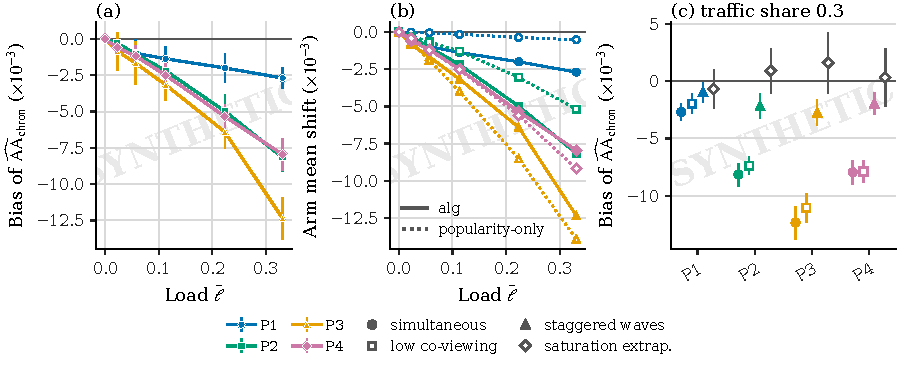
\includegraphics[width=0.94\textwidth]{figures/fig-sim-interference.pdf}
\caption{Synthetic data, E2: interference through shared popularity ($R=24$ paired replications; bars $\pm2$ SE). (a) Bias of the additive amplification relative to the reverse-chronological feed against the load $\bar\ell$, simultaneous design. (b) Shift in mean exposure of the algorithmic arm (solid) and the popularity-only arm (dotted); the reverse-chronological arm does not move. (c) Bias at traffic share $0.3$: simultaneous (load $0.33$), low co-viewing ($0.33$), staggered waves ($0.12$), and randomised-saturation extrapolation from shares $0.1$ and $0.3$.}\label{fig:sim-interference}
\end{figure}

\begin{figure}[tp]
\centering
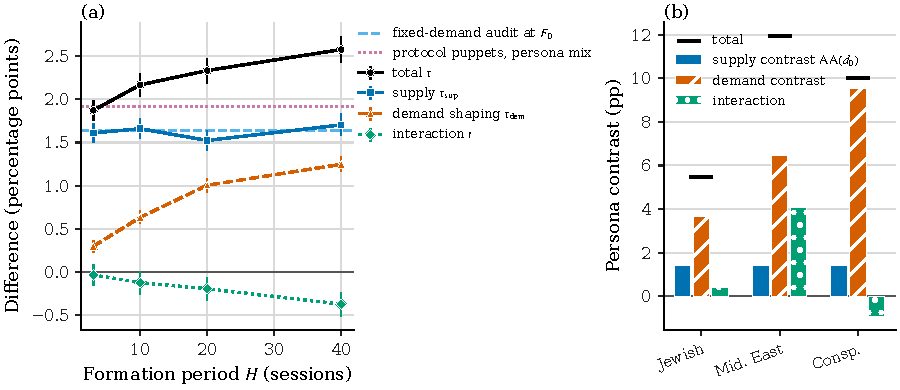
\includegraphics[width=0.94\textwidth]{figures/fig-sim-decomp.pdf}
\caption{Synthetic data, E3: the decomposition of \cref{thm:decomp}. (a) Components for $3{,}000$ synthetic users whose demand evolves, against the length $H$ of the formation period (reference: reverse-chronological; bars $\pm2$ SE over users). Lines: the fixed-demand audit at the initial demand $F_0$, and protocol puppets with the persona mix of the population. (b) Persona-contrast decomposition relative to P1 ($d_0$; protocol puppets, regime ND); black marks: total $\mu_{\mathrm{alg}}(d)-\mu_{\mathrm{ref}}(d_0)$.}\label{fig:sim-decomp}
\end{figure}

\begin{figure}[tp]
\centering
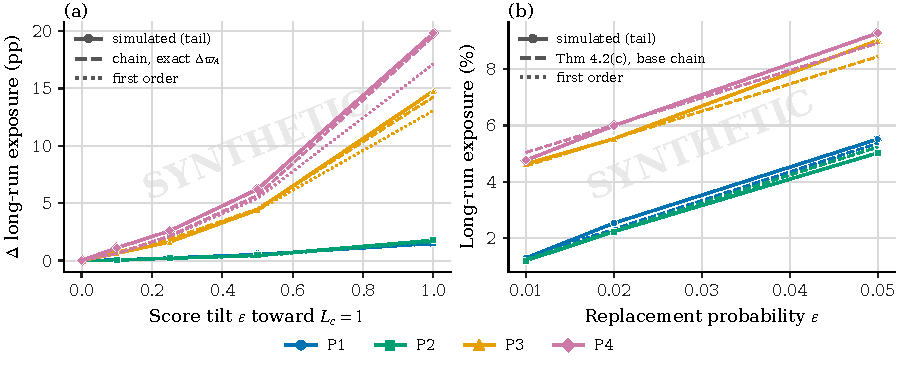
\includegraphics[width=0.94\textwidth]{figures/fig-sim-perturb.pdf}
\caption{Synthetic data, E4: perturbations of the chains of consumed items (algorithmic policy, $250$ naturalistic accounts per persona, common random numbers across $\varepsilon$). (a) Score tilt $\varepsilon$ toward items with $L_c=1$: simulated change in long-run exposure, the exact change between the estimated chains (\cref{thm:perturb}(a)), and its first-order term. (b) Replacement of the next item by an antisemitic one with probability $\varepsilon$: simulation, the closed form of \cref{thm:perturb}(c) from the base chain alone (dashed), and its first-order term $\varpi(\mathcal A)(1+\varepsilon\,\E_\varpi[T_{\mathsf A}])$ (dotted).}\label{fig:sim-perturb}
\end{figure}

\begin{figure}[tp]
\centering
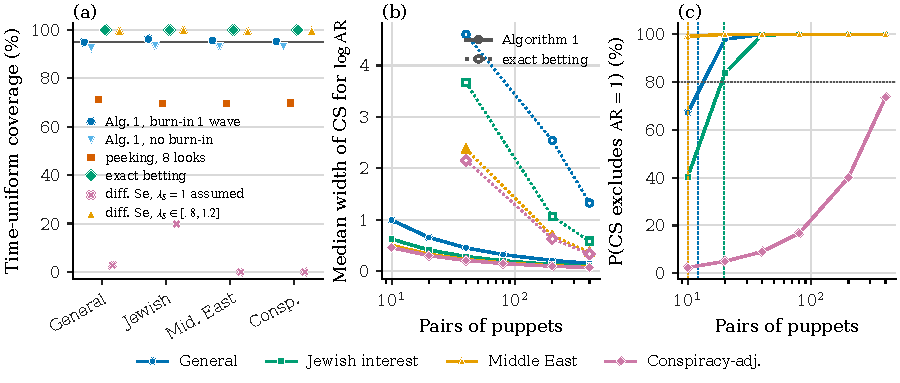
\includegraphics[width=0.94\textwidth]{figures/fig-sim-sequential.pdf}
\caption{Synthetic data, E5 (benchmark: conventional small-lab design, \cref{alg:sequential} on the confirmed-flagged statistic $Y_u$, waves of five pairs, ten sessions per puppet; $R=2{,}000$; exact betting $R=200$). (a) Time-uniform coverage at $\alpha=0.05$ over $80$ waves, with and without one burn-in wave; a fixed-sample interval recomputed after each of the first eight waves (peeking); exact betting; and, under DD, $\lambda_S=1$ assumed or the range $[0.8,1.2]$. (b) Median width for $\log\mathrm{AR}$: \cref{alg:sequential} (solid), exact betting (dotted). (c) Probability of excluding $\mathrm{AR}=1$; dashed verticals: the horizon $n_{\mathrm{seq}}$ of \cref{prop:power}(d), at least two waves (beyond the axis for P4).}\label{fig:sim-sequential}
\end{figure}

\begin{table}[tp]
\centering
\caption{Synthetic data, E1b and E2: checks of \cref{thm:identify,thm:misclass,prop:interference}. E1b: $R=2{,}000$ audits; error rates known unless stated; external validation with $n_1=300$ coded positives and $n_0=1{,}500$ coded negatives. Design effect: $S\sigma^2/\sigma^2_{\mathrm s}$ of \cref{thm:identify} for $S=10$ sessions. Sessions iid: variance that treats the sessions of a puppet as independent. Experiment buckets: every account has a persistent random shift (s.d.\ $1$) in the algorithm's weight on the engagement prior. s.d.\ of $\log\widehat{\mathrm{AR}}$: Monte Carlo, and the median over audits of the delta-method value; $\mathrm{cv}_{\Sp}$ as in \cref{sec:meas-misclass}. Interference block: E2, simultaneous design ($R=24$). There $\xi_\Delta$ is the largest $|\text{bias}|/\bar\ell$ over the grid of loads and $\zeta$ the largest second divided difference of the bias in the load, so the bound of part (a) holds by construction and is attained where the largest ratio occurs.}\label{tab:sim-checks}
\footnotesize
\setlength{\tabcolsep}{3pt}
\simfit{% Generated by code/make_figures.py from results/sim_results.json -- do not edit by hand.
% E1b: R = 2000 audits per configuration; known error rates (thm:identify) unless
% stated; external validation n1 = 300 coded positives, n0 = 1500 coded negatives.
\begin{tabular}{@{}lrrrr@{}}
\toprule
Quantity & General & Jewish interest & Middle East & Conspiracy-adj. \\
\midrule
\multicolumn{5}{@{}l}{\emph{Non-differential error, profiles as simulated (20 puppets per cell)}} \\
Design effect, alg; ref & 1.08; 0.96 & 1.07; 1.01 & 1.23; 1.04 & 1.10; 0.99 \\
Coverage AA: cluster-robust; sessions iid (\%) & 94.2; 94.8 & 94.6; 95.0 & 93.7; 92.8 & 94.2; 94.2 \\
Coverage $\log\mathrm{AR}$: cluster-robust; sessions iid (\%) & 94.5; 95.2 & 95.0; 95.2 & 93.8; 93.2 & 94.1; 94.3 \\
Naive AR; $\omega+(1-\omega)\mathrm{AR}$; true AR & 1.316; 1.325; 1.767 & 1.232; 1.231; 1.334 & 1.532; 1.534; 1.690 & 1.027; 1.033; 1.040 \\
External validation: s.d.\ of $\log\widehat{\mathrm{AR}}$, MC; delta (median) & 0.188; 0.159 & 0.062; 0.061 & 0.050; 0.050 & 0.039; 0.039 \\
\quad $\kappa_{\Sp}=v_{\Sp}^{1/2}/(J\mu_r)$ & 0.246 & 0.081 & 0.053 & 0.039 \\
\quad coverage $\log\mathrm{AR}$; AA (\%) & 94.2; 94.2 & 94.8; 95.3 & 95.0; 94.0 & 94.0; 94.1 \\
\addlinespace
\multicolumn{5}{@{}l}{\emph{Non-differential error, accounts in experiment buckets (20 puppets per cell)}} \\
Design effect, alg; ref & 3.47; 1.04 & 3.61; 1.02 & 5.65; 1.02 & 2.75; 1.03 \\
Coverage AA: cluster-robust; sessions iid (\%) & 93.0; 76.4 & 93.1; 75.6 & 93.0; 62.9 & 93.2; 82.5 \\
Coverage $\log\mathrm{AR}$: cluster-robust; sessions iid (\%) & 94.2; 85.0 & 93.7; 78.5 & 93.3; 69.3 & 93.2; 82.2 \\
\addlinespace
\multicolumn{5}{@{}l}{\emph{Differential error (coded false negatives), external validation, 20 puppets per cell}} \\
True AR; naive $\mathrm{AR}^{\mathrm{nv}}$; $\mathrm{AR}^{\mathrm{pool}}$ (eq.~\ref{eq:mc-diff}) & 1.784; 1.182; 1.494 & 1.353; 1.162; 1.254 & 1.780; 1.349; 1.487 & 1.053; 0.891; 0.861 \\
Corrected, pooled: median AR; coverage (\%) & 1.489; 73.5 & 1.250; 78.5 & 1.483; 15.7 & 0.861; 1.5 \\
Corrected, stratified by arm: median AR; coverage (\%) & 1.765; 97.9 & 1.348; 95.4 & 1.785; 95.0 & 1.050; 95.3 \\
\addlinespace
\multicolumn{5}{@{}l}{\emph{Interference (reference chron): \cref{prop:interference}(a) and (c)}} \\
$|$bias AA$|$; $\xi_\Delta\bar\ell$ at share 0.3 ($\times10^{-3}$) & 2.69; 7.20 & 8.16; 8.16 & 12.35; 12.35 & 7.95; 8.76 \\
$|$bias $\log\mathrm{AR}|$; ratio bound at share 0.3 & 0.088; 0.323 & 0.120; 0.146 & 0.095; 0.110 & 0.070; 0.087 \\
Extrapolation 0.05/0.1: $|$bias$|$; $\zeta\ell_1\ell_2/2$ ($\times10^{-3}$) & 0.61; 0.83 & 0.13; 0.94 & 0.19; 1.44 & 0.10; 1.08 \\
Extrapolation 0.1/0.2: $|$bias$|$; $\zeta\ell_1\ell_2/2$ ($\times10^{-3}$) & 0.73; 3.27 & 0.66; 3.70 & 0.13; 5.67 & 0.37; 4.23 \\
Extrapolation 0.1/0.3: $|$bias$|$; $\zeta\ell_1\ell_2/2$ ($\times10^{-3}$) & 0.69; 4.84 & 0.90; 5.49 & 1.59; 8.41 & 0.31; 6.27 \\
\bottomrule
\end{tabular}
}
\end{table}

\begin{table}[tbp]
\centering
\caption{Synthetic data: summary of E2--E5. E2: bias of the additive amplification relative to the reverse-chronological feed at traffic share $0.3$ ($R=24$; SE $0.4$--$0.7\times10^{-3}$), simultaneous design (load $0.33$), low co-viewing ($0.33$), staggered waves ($0.12$). E3: the ``real users'' are synthetic accounts whose demand evolves. E4: consumed items of naturalistic accounts, and the impression exposure of the same accounts. E4b: slate states of protocol puppets; long-run impression exposure in the second half of a $200$-step session, and its prediction by chains of true, observed and corrected slate states. E5 (benchmark): $R=2{,}000$ audits (MCSE about $0.5$ near $95\%$); coverage over all $80$ waves; peeking: fixed-sample interval after each of waves $1$--$8$; false detection: the sequence excludes $\mathrm{AR}=1$ when it is true; $n_{\mathrm{fix}}$, $n_{\mathrm{seq}}$ from $V_Y$ of \cref{prop:power}(d) for detecting $\mathrm{AR}\ne1$; last row: regime DD.}\label{tab:sim-designs}
\footnotesize
\setlength{\tabcolsep}{3pt}
\simfit{% Generated by code/make_figures.py from results/sim_results.json -- do not edit by hand.
\begin{tabular}{@{}lrrrr@{}}
\toprule
Quantity & General & Jewish interest & Middle East & Conspiracy-adj. \\
\midrule
\multicolumn{5}{@{}l}{\emph{E2: interference (reference chron, traffic share 0.3, load 0.33)}} \\
$\mathrm{AA}^0$ ($\times10^{-3}$) & 14.3 & 18.2 & 54.9 & 3.2 \\
Bias of $\widehat{\mathrm{AA}}$ ($\times10^{-3}$) & $-$2.7 & $-$8.2 & $-$12.3 & $-$8.0 \\
\quad with low co-viewing & $-$2.0 & $-$7.4 & $-$11.1 & $-$7.9 \\
\quad with staggered waves & $-$1.0 & $-$2.2 & $-$2.8 & $-$2.0 \\
\addlinespace
\multicolumn{5}{@{}l}{\emph{E3: real users, formation $H=40$ sessions (pp): $\tau=2.58$, $\tau_{\mathrm{sup}}=1.70$, $\tau_{\mathrm{dem}}=1.25$, $\iota=-0.37$; audit at $F_0$: 1.64}} \\
\addlinespace
\multicolumn{5}{@{}l}{\emph{E4: Markov model, algorithmic policy (consumed items, \%)}} \\
$e_{20}$ predicted / simulated & 0.28 / 0.28 & 0.26 / 0.26 & 3.16 / 3.16 & 3.62 / 3.60 \\
$e_{200}$ predicted / simulated & 0.30 / 0.38 & 0.28 / 0.22 & 3.36 / 3.54 & 3.84 / 3.89 \\
$\kappa_{\mathcal A}$; Kemeny $K$ & 0.50; 2.07 & 0.51; 1.98 & 0.51; 2.04 & 0.52; 2.17 \\
\addlinespace
\multicolumn{5}{@{}l}{\emph{E5: \cref{alg:sequential}, reference chron, waves of 5 pairs, $\alpha=0.05$ unless stated}} \\
True AR & 1.79 & 1.33 & 1.67 & 1.04 \\
Time-uniform coverage, burn-in 1 wave; none (\%) & 95.0; 92.6 & 96.2; 93.5 & 95.7; 93.3 & 95.2; 93.2 \\
\quad peeking, waves 1--8 (\%) & 71.2 & 69.8 & 69.5 & 69.8 \\
Null AR$=1$: false detection by wave 8, Alg.~1; peeking (\%) & 2.9; 30.3 & 2.1; 29.2 & 2.5; 29.8 & 3.4; 33.0 \\
P(excludes AR$=1$) by wave 8 (\%) & 100.0 & 99.8 & 100.0 & 9.0 \\
$n_{\mathrm{fix}}$; $n_{\mathrm{seq}}$ from $A_Y$ (pairs) & 6; 12 & 10; 20 & 2; 4 & 267; 512 \\
Power at $n_{\mathrm{fix}}$ (fixed); by horizon (sequential) & 0.87; 0.92 & 0.85; 0.85 & 0.93; 1.00 & 0.82; -- \\
Differential Se: $\lambda_S$; coverage with $\lambda_S{=}1$; with $[0.8,1.2]$ (\%) & 0.86; 2.8; 99.6 & 0.93; 19.8; 100.0 & 0.83; 0.0; 99.4 & 0.82; 0.0; 99.6 \\
\bottomrule
\end{tabular}
}
\end{table}
